% Created 2019-01-18 Fri 08:08
% Intended LaTeX compiler: pdflatex
\documentclass[11pt]{article}
\usepackage[utf8]{inputenc}
\usepackage[T1]{fontenc}
\usepackage{graphicx}
\usepackage{grffile}
\usepackage{longtable}
\usepackage{wrapfig}
\usepackage{rotating}
\usepackage[normalem]{ulem}
\usepackage{amsmath}
\usepackage{textcomp}
\usepackage{amssymb}
\usepackage{capt-of}
\usepackage{hyperref}
\usepackage[top=0.5in]{geometry}
{\setlength{\parindent}{0cm}
\author{Kayvan Kazeminejad}
\date{\today}
\title{RSong Story-Board}
\hypersetup{
 pdfauthor={Kayvan Kazeminejad},
 pdftitle={RSong Story-Board},
 pdfkeywords={},
 pdfsubject={},
 pdfcreator={Emacs 26.1 (Org mode 9.1.13)}, 
 pdflang={English}}
\begin{document}

\maketitle
\begin{center}
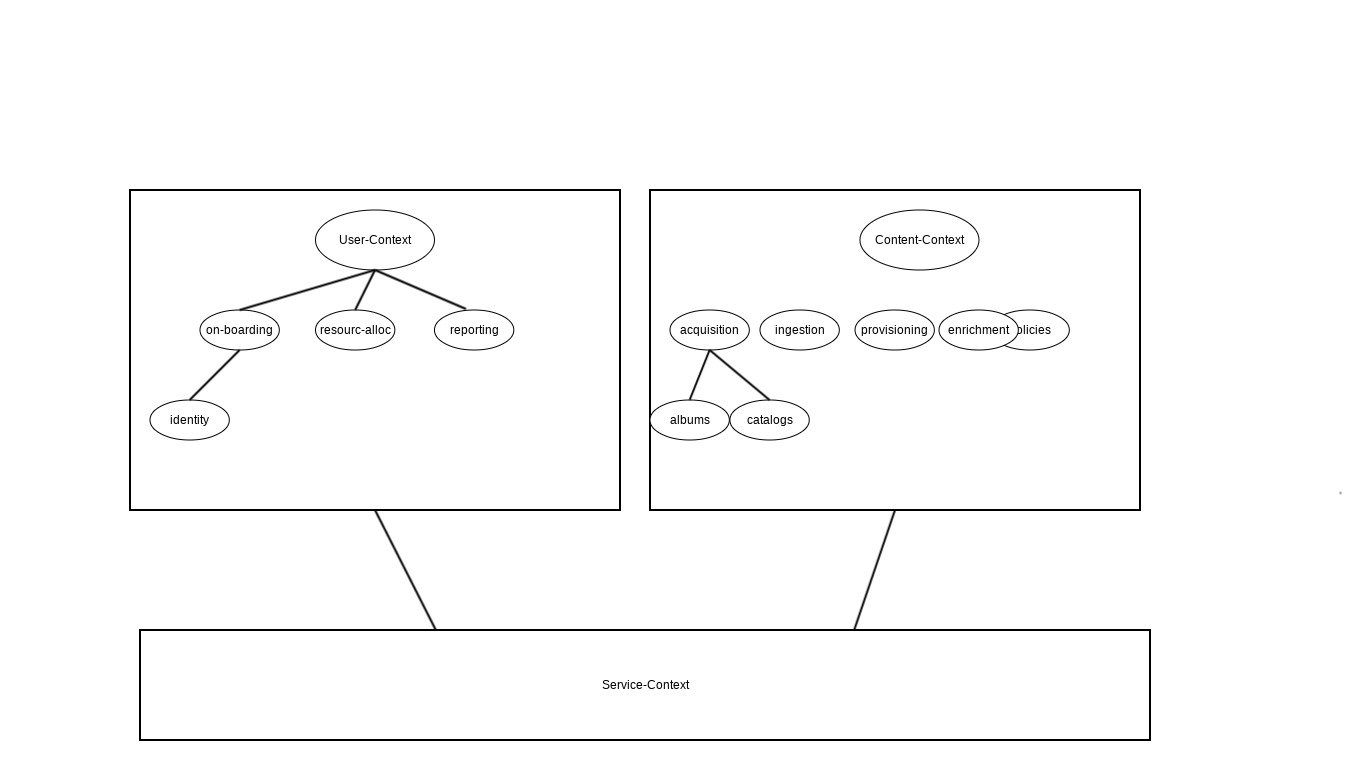
\includegraphics[angle=0,width=10cm]{./design/story-board.jpeg}
\end{center}

\section*{RSong Story Board}
\label{sec:orgdc59b1e}
The purpose of this section is to provide a high level coherent definition for 
\begin{itemize}
\item RSong
\item RSongs purpose
\item the problem space RSong is addressing
\end{itemize}

\subsection*{RSong stories}
\label{sec:org59e6adf}
The purpose of this section is to divides up the system into Bounded Contexts, each of which can have a unified model - essentially a way of structuring MultipleCanonicalModels.
This section
\begin{itemize}
\item User-context
\item Content-Context
\item Service-Context
\end{itemize}

\subsubsection*{User-Context}
\label{sec:orgb047251}
This section encapsulates, and defines the specific responsibilities of the user-context to the model.

User context is fragmented to:
\begin{itemize}
\item providers
\item consumers
\end{itemize}

\begin{itemize}
\item Providers
\label{sec:org0f2aca8}
Content providers are artists or catalog owners. Stories are:
\begin{itemize}
\item on-boarding
\item reporting
\item monetization
\end{itemize}

\begin{itemize}
\item on-boarding
\label{sec:org567c974}
\begin{itemize}
\item identity
\item individual content
\item catalog owners
\end{itemize}

\item reporting
\label{sec:org280f01d}
TBD: Provide definition 

\item monetization
\label{sec:org2d589b4}
TBD: Provide definition 
Smart contract related
\end{itemize}

\item Consumers
\label{sec:org2fd4db9}
Content consumers are the viewers of the system.  Stories are:
\begin{itemize}
\item on-boarding
\item reporting
\item resource allocations
\end{itemize}

\begin{itemize}
\item on-boarding
\label{sec:org1858654}
TBD: Provide definition 

\item reporting
\label{sec:orgc6e9514}
report on token consumption

\item resource allocations
\label{sec:orgcfee835}
token allocation/consumption
\end{itemize}
\end{itemize}

\subsubsection*{Content-Context}
\label{sec:org97fc8c0}
This section encapsulates, and defines the specific responsibilities of the context-context to the model.

Contents are RSong related assets, \textbf{Songs}., songs.  Stories are:
\begin{itemize}
\item acquisition
\item ingestion
\item provisioning
\item enrichment
\item policies
\end{itemize}

\begin{itemize}
\item acquisition
\label{sec:org0aaa352}
Content acquisition the entry of assets to the RSong system. The flow is: 

acquisition -> ingestion -> provisioning

acquisition is fragmented to: 
\begin{itemize}
\item album
\item catalog
\end{itemize}
Once assets are acquired they
\begin{itemize}
\item validation
\item verification
\end{itemize}
\begin{itemize}
\item albums
\label{sec:orgd23693b}
TBD: Provide definition 

\item catalog
\label{sec:org0c93c2f}
TBD: Provide definition 

\item validation
\label{sec:org4e920bb}
TBD: Provide definition 

\item verification
\label{sec:org4a43c8d}
TBD: Provide definition
\end{itemize}

\item ingestion
\label{sec:orgd419dc2}
ingestion occurs where we have complete asset.

\item provisioning
\label{sec:org2bbb81c}
make an asset searchable/playable

\item policies
\label{sec:org0480c74}
TBD
\end{itemize}

\subsubsection*{Service-Context}
\label{sec:orgfbb77bd}
This section encapsulates and defines functionality and feature the system provides
\end{document}